\documentclass[12pt, twoside]{article}
\usepackage{jmlda}
\usepackage{graphicx} 
\graphicspath{ {./figures/} }
\usepackage{caption}
\usepackage{subcaption}
\usepackage{subfig}
\newcommand{\hdir}{.}
\renewcommand{\baselinestretch}{1.35}

\begin{document}
\English
\title
	[] % short title for page headings, not necessary if a full title fits the headings
    { Learning co-evolution information with natural language processing for protein folding problem} % full title
\author
	[F.\,S.~Author] % short list of the authors (<= 3) for page headings, is necessary only if the full list does not fit the headings
	{F.\,S.~Author, F.\,S.~Co-Author, and F.\,S.~Name} % full list of the authors, presented in the table of contetns of the issue
    [Egor Zverev$^1$, Sergei Grudinin$^2$, and Ilia Igashov$^{1, 2}$] % list of the authors presented in the title page of the article, is necessary only if it differs from the full list of the authors in braces, i.e. '{' and '}'
\email
    {zverev.eo@phystech.edu; sergei.grudinin@inria.fr; igashov.is@phystech.edu}
\thanks
    {}
\organization
    {$^1$Organization, address;
     $^2$Organization, address}
\abstract
    {Co-evolution information is crucial for building protein sequence descriptors. Its computation is traditionally based on Multiple Sequence Alignments. Applications of MSA are limited, for instance, it fails for sequences with shallow alignment. This work investigates pre-trained language models as potential alternatives to MSA. The main focus is on fold classification problem. The authors examine several  state-of-the-art  methods  and  modify  them  by  replacing  MSA-based  feature-generation parts with pre-trained LMs. They compare language models and MSA in their ability to extract sequence evolution information. The performance of models is compared using TOP1-accuracy score.

		
	\noindent
    	\textbf{Keywords}: \emph{protein fold classification; co-evolution, feature generation; transformers; BERT;  }}




%these fields are filled in by the journal editors
\doi{10.21469/22233792}
\receivedRus{01.01.2017}
\receivedEng{January 01, 2017}

\maketitle
\linenumbers

\section{Introduction}
\noindent %this command is placed at the beginning of the first sentence of each paragraph/section only.




Protein properties are determined by its shape, which is specified by its amino acid sequence \cite{cellbiology}. Therefore it is important to learn how to analyze this sequence.
The first step is constructing protein sequence descriptors. Ideally the descriptors contain co-evolution information[...]. This information is obtained by searching for homologues of the protein in large databases and computing multiple sequence alignment (MSA) on it. This model requires significant computational effort. Alignment databases are finite. If for a given sequence there are no matches in the database, MSA-based methods fail to produce reliable results. 
 It does not guarantee precise results since it fully relies on finite databases. MSA-based methods fail for sequences with shallow alignment.

 Co-evolution-based methods assume[...] that a mutation of one amino acid leads to mutations of others. Therefore, given an amino acid sequence it is natural to look for other similar sequences. That is performed with MSA \cite{co-evolution}. This method fails when we are dealing with the sequences that did not evolve a lot. They have shallow alignments. That means there are only a few similar sequences in the database. Therefore, information extracted from these alignments is insignificant. 

The authors propose to analyse pre-trained language models (LMs)  \cite{Elnaggar} as potential alternative to traditional MSA-based models. It is assumed that protein sequences are not random \cite{evolution-not-random}, There is structure in amino acid sequences. Therefore, a set of all amino acids could be seen as a language with complicated inner rules. BERT \cite{bert} learns the structure of any abstract language. We assume that by learning amino acids structure, BERT will be able to implicitly learn co-evolution information.

Our main aim is to study the efficiency of pre-trained LMs in application to the fold classification problem.  To start with, we study the state-of-the-art method DeepSF \cite{DeepSF}. It solves the protein fold classification problem.  By replacing its MSA-based feature-generation part with a pre-trained LM, we study how NLP approach affects learning the fold-related information.  The whole framework is schematically represented in Figure 1. Further, we perform the same with other fold classification algorithms \cite{Villegas, DeepFrag}
as well as with end-to-end protein structure prediction methods \cite{Kandathil, Xu2020.10.12.336859}.

\begin{figure}[htp]
    \centering
    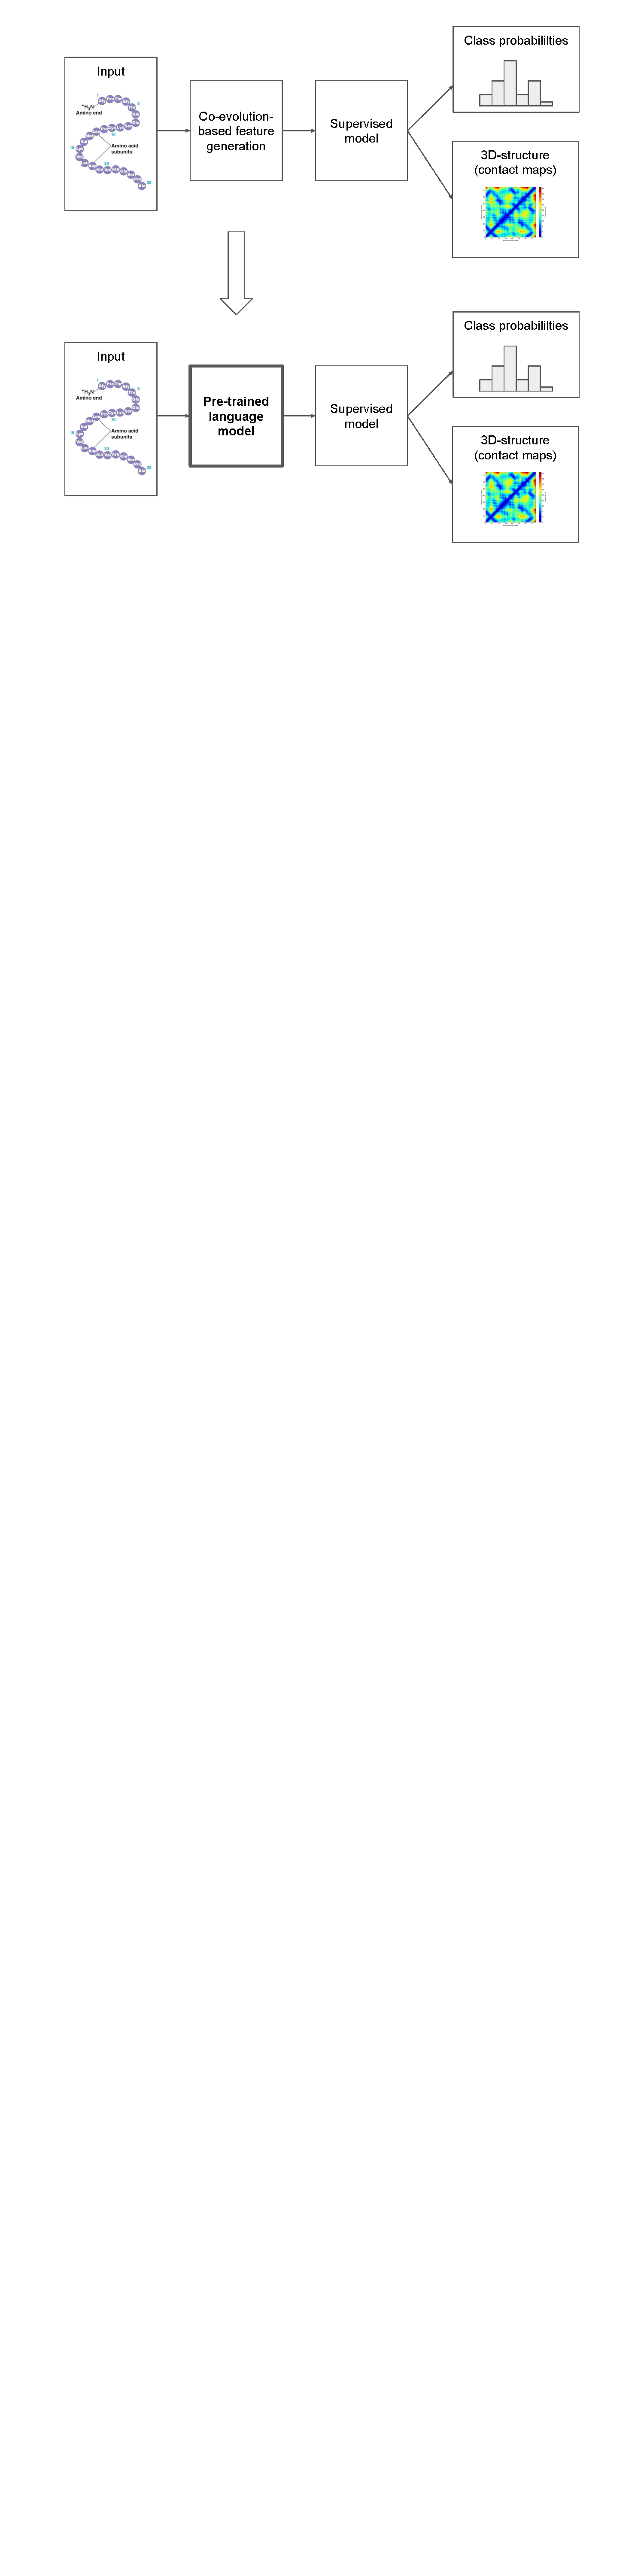
\includegraphics[width=10cm]{figures/figure1.pdf}
    \caption{The main framework}
\end{figure}
\section{Problem statement}
\noindent
Proteins that share similarities in their structure are  divided into classes -- folds \cite{Schaeffer2011}. In this work we investigate a fold classification problem.

\paragraph{General description}
\noindent
  

We denote $Y$ a set of all known classes, $A$ a set of all proteins with known folds and  $f: A \rightarrow Y$ a mapping between proteins and their classes. 

Suppose, $x \not\in A$ is a protein with unknown fold. We aim to build a model capable of classifying $x$ as an element of one of the present classes, extending $f$ on the set $A \cup \{x\}$. 

\paragraph{Feature generation }
\noindent

In the fold classification problem $x_i$ represents $i$-th protein description in  $D$-dimensional space. However, initially each protein is described by its amino acid sequence. Let $\Sigma$ be the 20-letter alphabet of acid sequences.  

There is a set $A = \{a_i \in \Sigma^+\}_{i = 1}^n$ of protein sequences. Let $$g_{\theta, D}: \Sigma^+ \rightarrow \mathbb{R}^D$$ be an embedding of space of acid sequences into $D$-dimensional set of descriptors. These embeddings are parameterized  by $\theta$.

We separate $A$ into training and validation set. Training set is used to formulate fold classification problem. Validation set is used to formulate feature generation problem. 

$$A = A_{\text{train}} \cup A_{\text{val}}$$

Protein sequence descriptors are generated using $g_{\theta, D}$ as $x_i = g_{\theta, D}(a_i)$ 

\paragraph{Fold classification problem}
\noindent

Suppose there is a given set of pairs $S = \{ (x_i, Y_i)\}_{i = 1}^n$ where $ x_i \in \mathbb{R}^D$ denotes the sequence descriptor of $i$-th protein and $$Y_i \in \mathbb{Y} = \{ (1, 0, ..., 0), (0, 1, 0, ..., 0) .... (0, ..., 0, 1) \}$$ denotes the i-th protein known class, $|\mathbb{Y}| = m$

We separate $S$ into training and validation set. Training set is used to formulate fold classification problem.  

$$S = S_{\text{train}} \cup S_{\text{val}}$$

Let $W = \{(w_1, ..., w_m)| w_i \in \mathbb{R}^D\}$ be a space of parameters for classification models. Let $g_w$ be a model parameterized by $w$.
We use $e_k$ to denote a vector with 1 on $k$-th position, with zeros on all other positions
\[
\begin{matrix}
e_{k} = &
        &[0,\ldots,0,&1,&0,\dots,0].\\
        &&&\uparrow&      \\
        &&&k&           
\end{matrix}
\]
We work under the following assumption:  

$$P_w(Y = e_k| x) = \frac{exp(x^Tw_k)}{\sum_j exp(x^t w_j)}$$
Let $p_{w, x}(y)$ be discrete density of $Y$, $L_{Y, x}(w)$ be likelihood function of $Y$.  

$$p_{w, x}(y) = \prod_{d = 1}^{m} (P_w(Y = e_d| x))^{y_d}$$, 

$$L_{Y, x}(w) = \prod_{i = 1}^{n} p_{w, x}(Y_i)$$

Given $S_{train}$, classification problem is a maximization of likelihood on training set: 

$$L_{train}(w) = L_{Y_{train}, x_{train}}(w) \rightarrow \max\limits_{w \in W}$$

\paragraph{Feature generation problem}
\noindent

For fixed $\theta, D$ and descriptors $x_i$ we denote $$\hat{w} = \argmax\limits_{w \in W} L_{Y_{train}, x_{train}}(w).$$. 

Feature generation problem is a maximization of likelihood function on validation set:  

$$L_{Y_{val}, x_{val}}(\hat{w}) \rightarrow \max\limits_{\theta, D}$$

\paragraph{Overview}
\noindent

The problem of determining proteins' class is separated into two parts: first, we encode amino acid sequences as $D$-dimensional descriptors, then these descriptors are used to train a prediction model.  


\section{Computational experiment}

The goal of our experiments is to verify that BERT is capable of extracting important features from the given amino acid sequences. For this we will use pre-trained AlBert\cite{ProtBert} model to generate these features and then train our own neural networks to solve fold classification problem. 

\paragraph{Data}
\noindent
We use SCOP2 \cite{SCOP2FST, SCOP2SND} dataset. It contains information about proteins whose structure is already known. All the proteins in the database have classes assigned to them (folds).  At present, there are 1517 known folds \cite{SCOP2SND}. The number of proteins contained in each fold is less than 50 for most of the folds. Detailed histogram is represented in Figures 2, 3. 

\begin{figure}[htp]
    \centering
    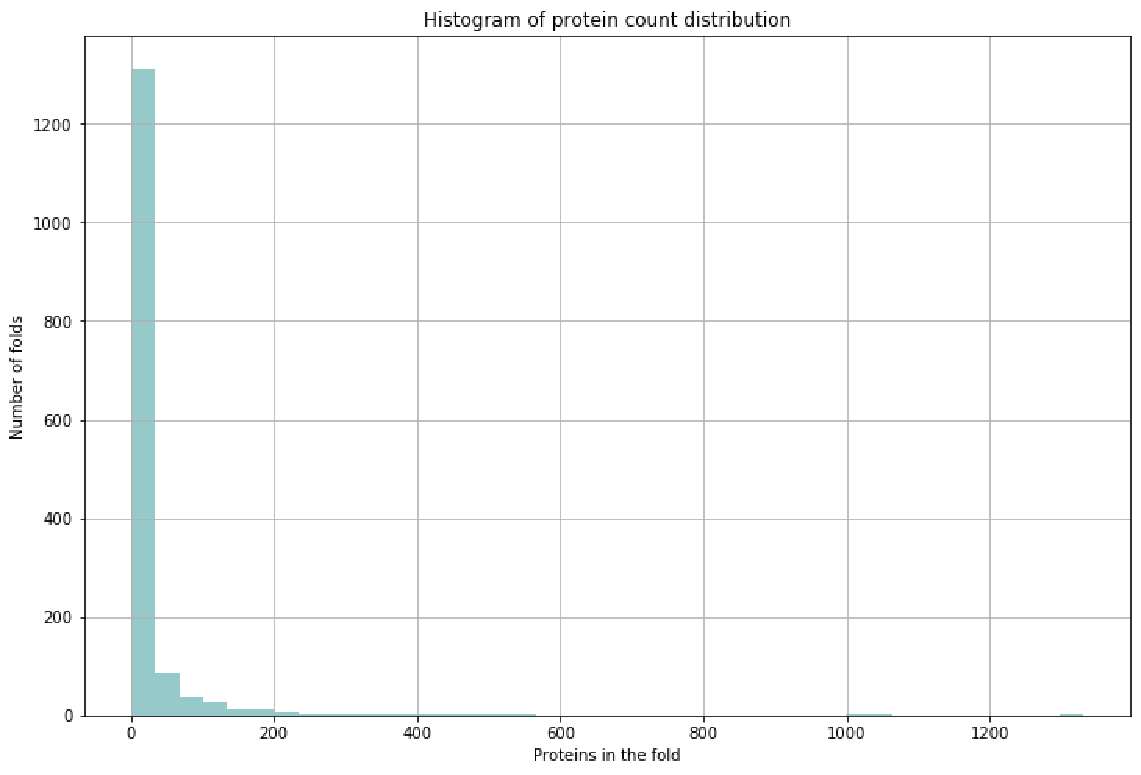
\includegraphics[width=10cm]{figures/figure2.pdf}
    \caption{Protein count histogram}
\end{figure}

\begin{figure}[htp]
    \centering
    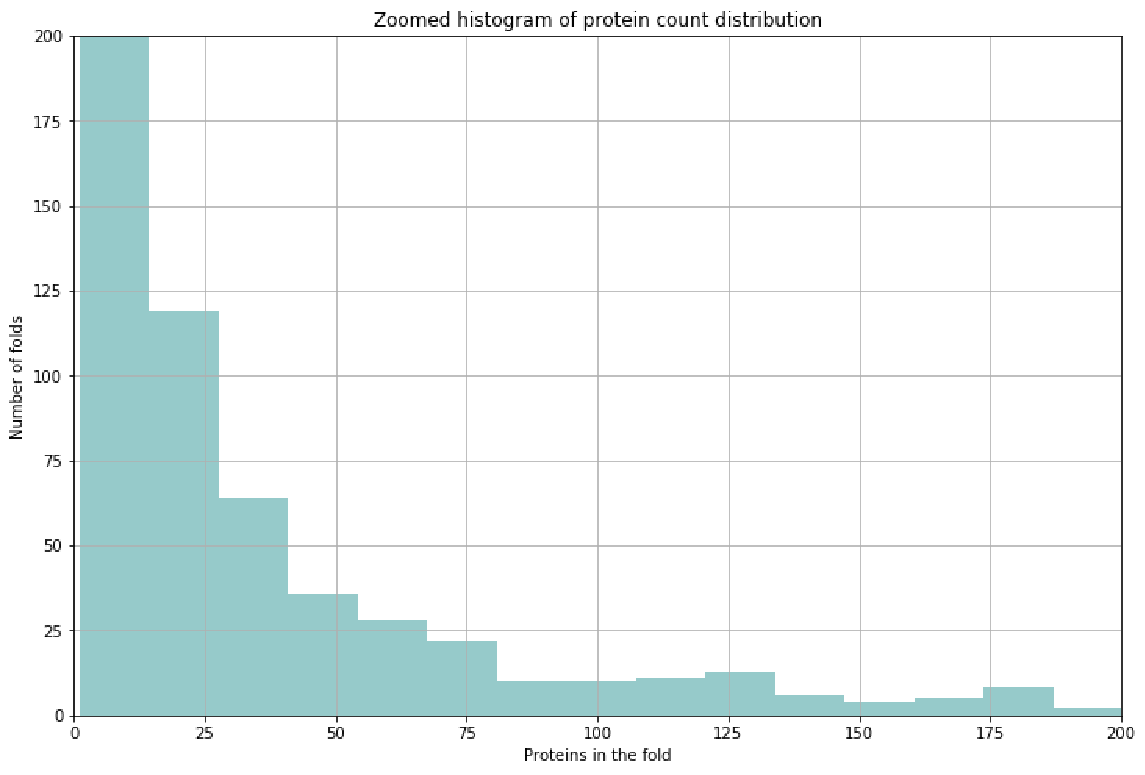
\includegraphics[width=10cm]{figures/figure3.pdf}
    \caption{Protein count zoomed histogram}
\end{figure}

In SCOP2 proteins are represented by their amino acid sequences. Each sequence is stored as a string in the 20 letter alphabet and an ID. The length of the string varies mostly between 25 and 500 from protein to another. The length diagram is represented on Figure 2. Search by ID allows database users to extract information about target proteins, including their fold classes. 

\begin{figure}[htp]
    \centering
    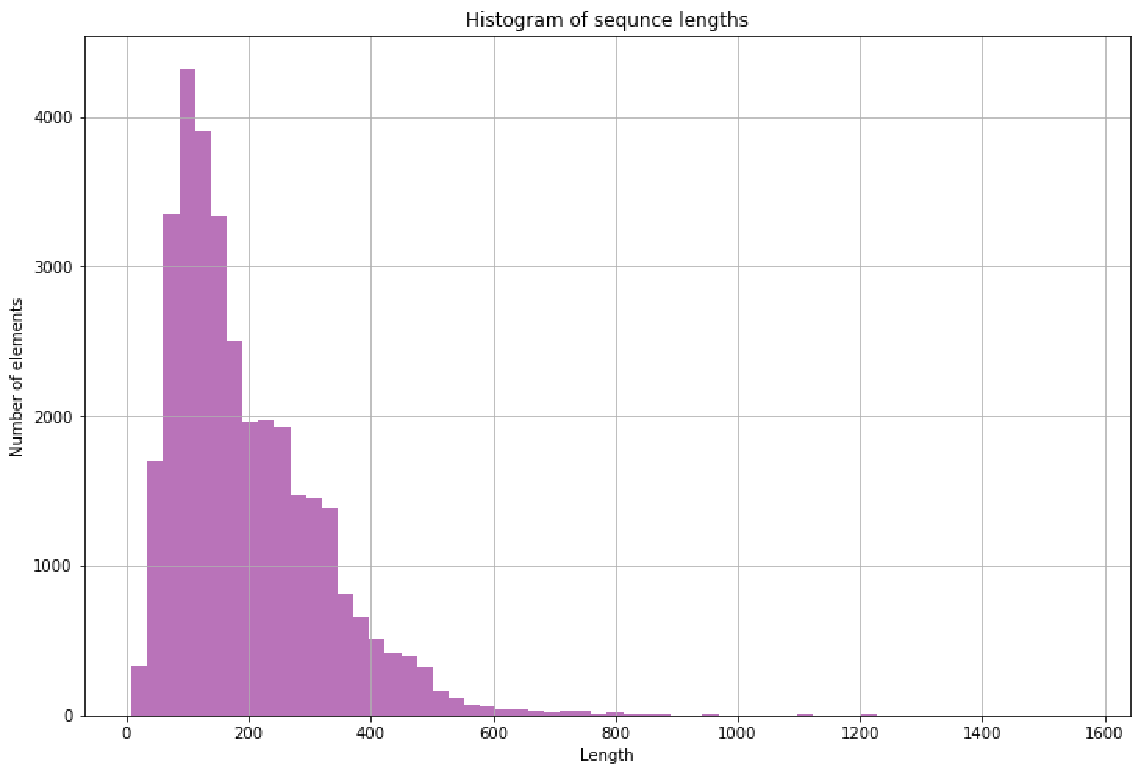
\includegraphics[width=10cm]{figures/figure4.pdf}
    \caption{Sequence length histogram}
\end{figure}


\paragraph{Baseline solution}
\noindent
Our solution is a modification of the DeepSF \cite{DeepSF} method. The designers of DeepSF use PSI-BLAST\cite{PSIBLAST} to generate features from MSA  as well as SCRATCH \cite{SCRATCH} to extract secondary structure (3 classes) and solvent accessibility (2 classes).  In the core of this classification method PSI-BLAST is used during the first stage of prediction \cite{SCRATCH}. 

Hoe et al. then use these features as an input to the deep convolutional neural network. The depth of CNN used in DeepSF is 10. The output of the model is a vector of fold probabilities. Fold with the maximal probability is accepted as a target protein fold. 

\paragraph{Proposed solution}
\noindent

DeepSF feature generation is entirely based on MSA. The main point of this work is to suggest another approach to feature generation which is independent of MSA. 

We apply BERT to the language of amino acids. We take the representation of acid sequences BERT creates as a new set of features. Then we train DeepSF model on these features.

It shall be noted that we do not reject co-evolution information in our research. Instead of directly applying MSA we let BERT learn information about amino acid language. We suppose that the model learns evolution information implicitly.

\paragraph{Evaluation}
\noindent
We use standard cross-validation procedure to compute accuracy of our model. We then compare it to the accuracy score of DeepSF method based on MSA feature generation as well as several other state-of-the-art techniques. 

\section{Experiment details}
Though the data is available for 1517 classes, during the experiments we approached the problem slowly. First, we solved a classification problem for 2 classes, then for 10 classes.

\paragraph{First experiment}
\noindent In this experiment we took two balanced classes. They contain 66 and 80 elements respectively. The distributions of their sequence length are similar. They are displayed on figure 5. We used a model that consists of two essential layers - 30-max-pooling followed by a linear layer. Using this architecture we achieved 93\% score on validation data. The architecture and training curves are represented on figures 6 and 7.  

The architecture presented here is the simplest possible one - it contains max-pooling layer to transform input to fixed size and FC layer for classification. Motivation for this experiment is to verify whether features extracted by BERT are meaningful.

\begin{figure}[htp]
    \centering
    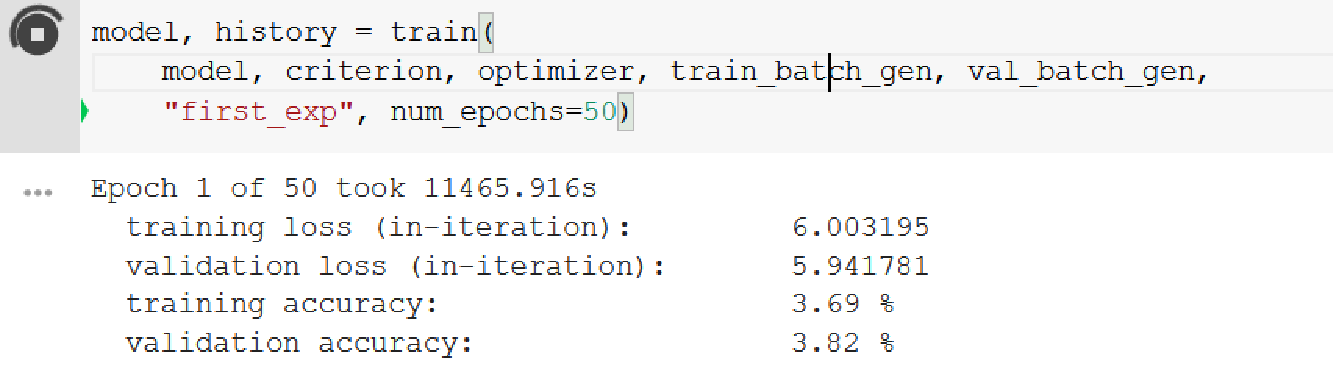
\includegraphics[width=10cm]{figures/figure5.pdf}
    \caption{Sequence lengths of two folds}
\end{figure}

\begin{figure}[htp]
    \centering
    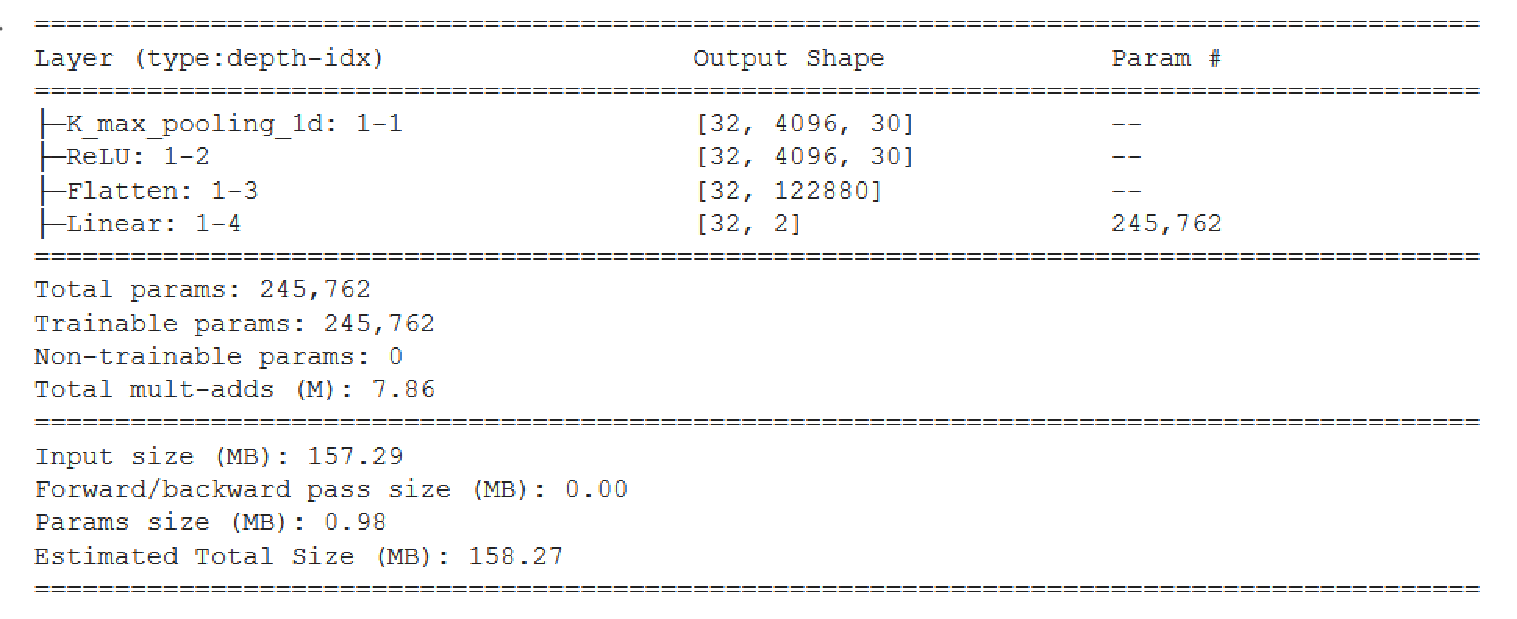
\includegraphics[width=12cm]{figures/figure6.pdf}
    \caption{Experiment 1 architecture}
\end{figure}
\begin{figure}[htp]
    \centering
    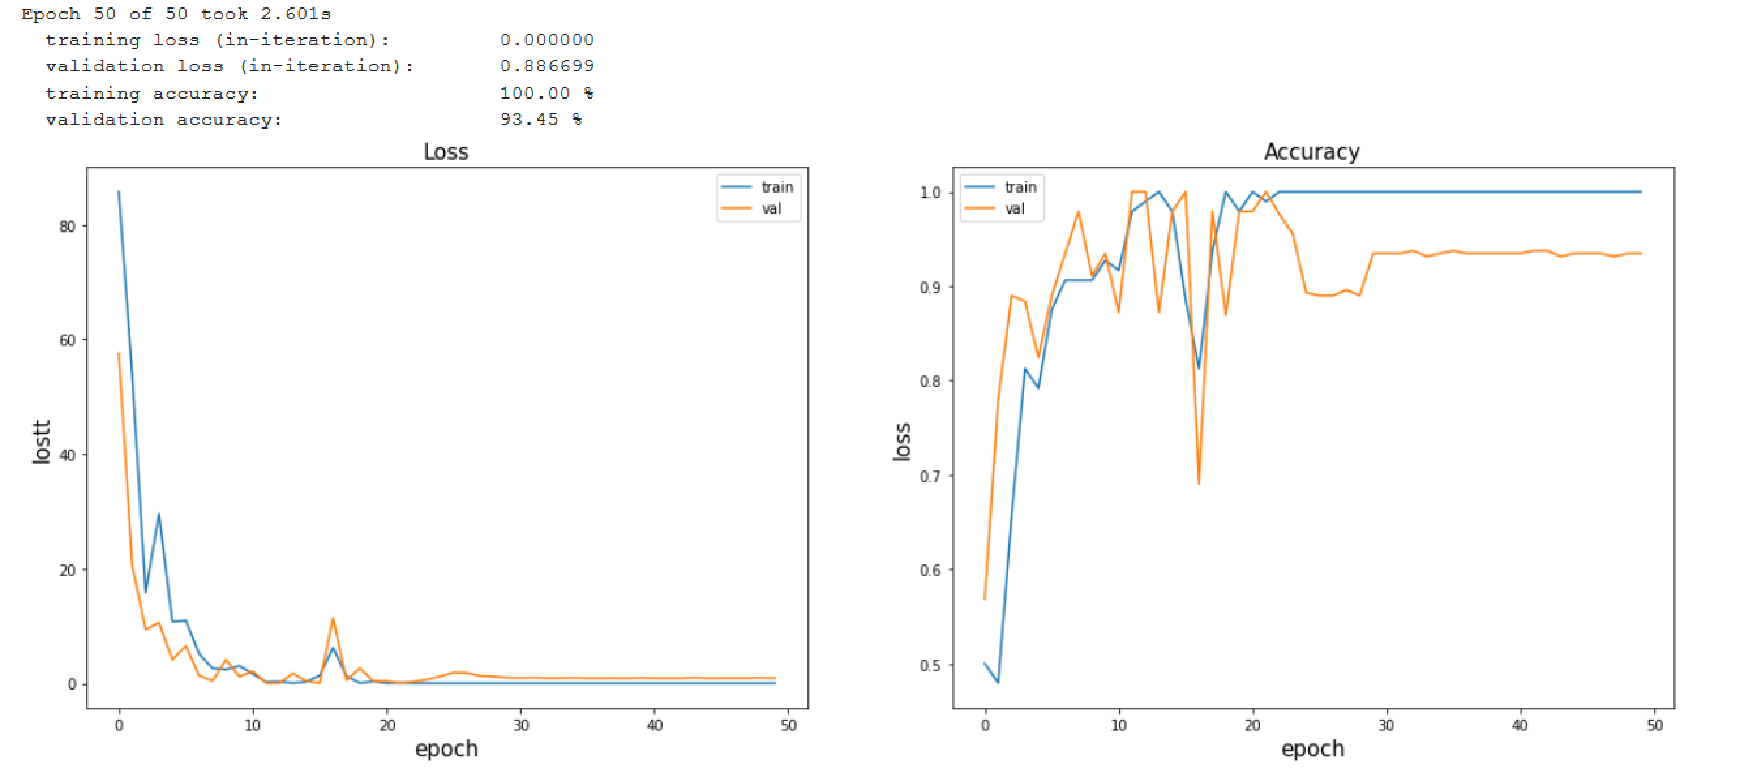
\includegraphics[width=18cm]{figures/figure7.pdf}
    \caption{Experiment 1 training curve}
\end{figure}

\paragraph{Second experiment}
\noindent
We decided to use exactly the same architecture for 10-fold classification problem. Our experiments show that increasing the k hyper-parameter in k-max-pooling layer improves the quality of the model. We chose k = 60. It allowed us to reach 95\% accuracy on validation and 93\% accuracy on test samples. The training curve is represented on figure 8.   

The second experiment is an extension of the first one. Its goal is to validate that simple 2-layer architecture could deal with more complicated classification problem.

\begin{figure}[htp]
    \centering
    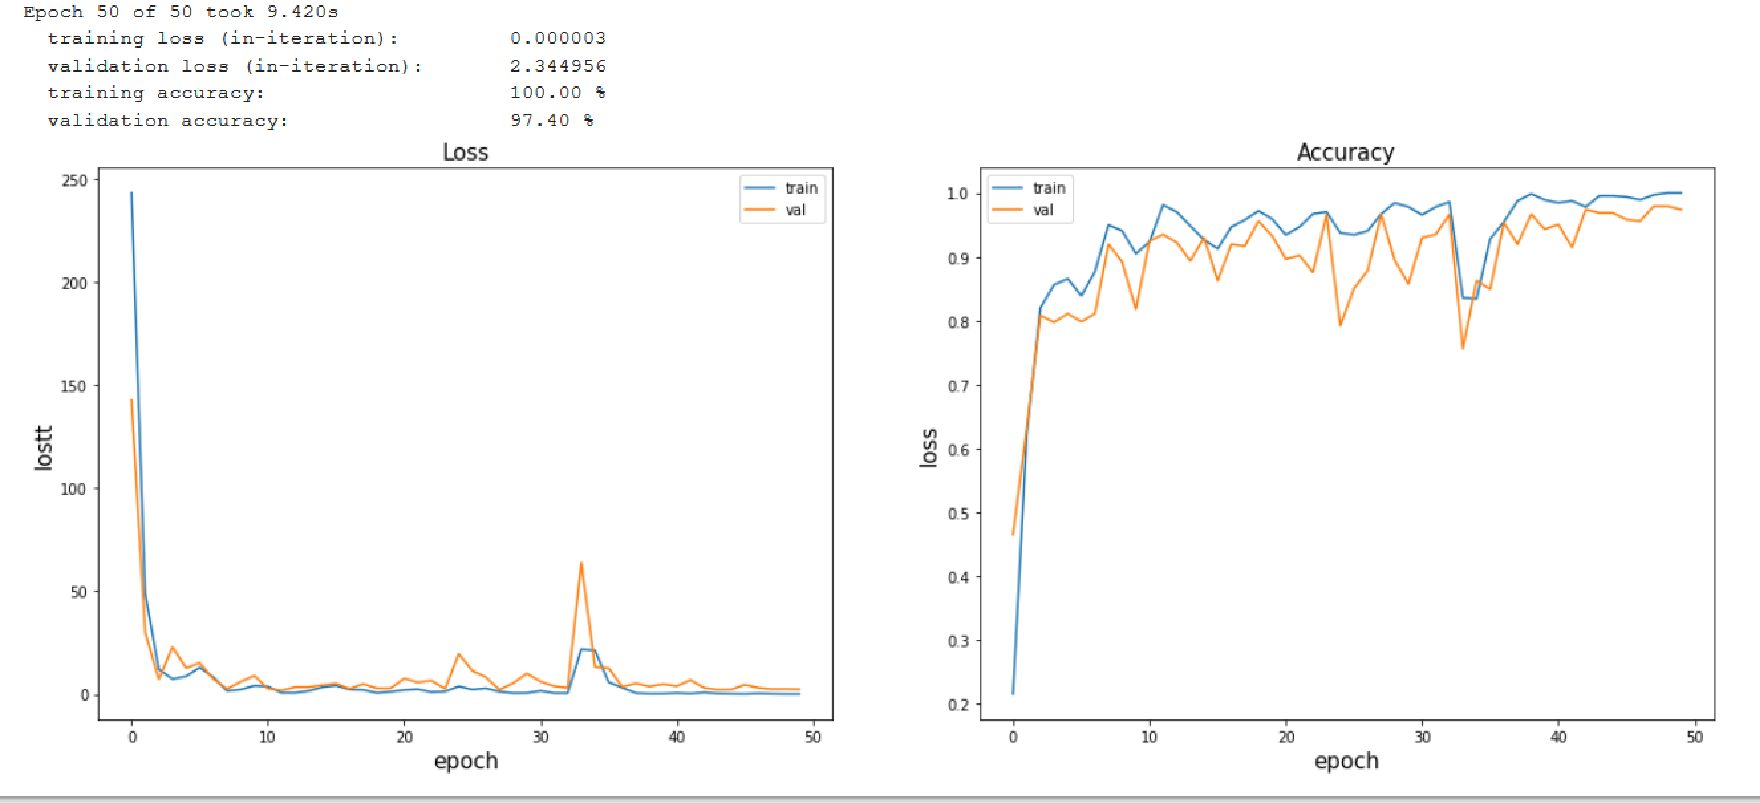
\includegraphics[width=10cm]{figures/figure8.pdf}
    \caption{Experiment 2 training curve}
\end{figure}



\section{Feature work}
In this paper we investigated only classification problem for at most classes. In the future we would like to extend our experiments for 1517-fold classification problem and compare the results.

Here we used BERT as a "black box". We generated features with BERT and used them as an input for another model. The desired improvement here would be to learn how to extract attention mechanisms from BERT, possibly gaining more co-evolution information in the process.


\section{Results}
\noindent

Conducted experiments show that BERT successfully captured the structure of the protein sequence language (or at least its part). We managed to solve 10-fold classification problem with 93\% accuracy.

Therefore, BERT is capable of extracting crucial information from the sequences of amino acids.

%please do not change the name of this section if it is present

%%%% please specify doi of the cited item if possible, see~\bibitem{article}
%%%% Crossref doi of the item can be retrieved at http://www.crossref.org/guestquery/
\bibliographystyle{plain}
\bibliography{Zverev2020CoevolutionFromLMs}

%begin{thebibliography}{99}



% \bibitem{book}
% 	\BibAuthor{Goossens,~M., F. Mittelbach, and A.~Samarin}. 1994.
% 	\BibTitle{The \LaTeX\ companion}.
% 	2nd ed.
% 	Reading, MA: Addison-Wesley. 528 p.

% \bibitem{article}
% 	\BibAuthor{Zagurenko,~A.\,G., V.\,A.~Korotovskikh, A.\,A.~Kolesnikov, A.\,V.~Timonov, and D.\,V.~Kardymon}. 2008.
% 	Tekhniko-ekonomicheskaya optimizatsiya dizayna gidrorazryva plasta
% 	[Technical and economic optimization of the design of hydraulic fracturing].
% 	\BibJournal{Neftyanoe Khozyaystvo} [Oil Industry] 11(1):54--57.
% 	\BibDoi{10.3114/S187007708007}. (In Russian)

% \bibitem{webArticle}
% 	\BibAuthor{Blaga,~P.\,A.} 2007.
% 	Commutative Diagrams with XY-pic II. Frames and Matrices.
% 	\BibJournal{PracTEX J.}  4.
% 	Available at: \BibUrl{https://tug.org/pracjourn/2007-1/blaga/blaga.pdf}
%     (accessed February 20, 2007).

% \bibitem{webResource}
% 	XYpic.
% 	Available at: \BibUrl{http://akagi.ms.u-tokyo.ac.jp/input9.pdf}
% 	(accessed April 09, 2015).

% \bibitem{inproceedingsRus}
% 	\BibAuthor{Usmanov,~T.\,S., A.\,A.~Gusmanov, I.\,Z.~Mullagalin, R.\,Yu.~Mukhametshina, A.\,N.~Chervyakova, and A.\,V.~Sveshnikov.} 2007.
% 	Osobennosti proektirovaniya razrabotki mestorozhdeniy s primeneniem gidrorazryva plasta
% 	[Features of the design of field development with the use of hydraulic fracturing].
% 	\BibJournal{6th Symposium (International) ``New Energy Saving Subsoil Technologies and the
% 	Increasing of the Oil and Gas Impact'' Proceedings}.
% 	Moscow:~Publisher. 267--272. (In Russian)
	   	
% \bibitem{inproceedingsEng}
%     \BibAuthor{Author,~N.} 2009.
%     Paper title.
%     \BibJournal{10th Conference (International) on Any Science Proceedings}.
%     Place of publication: Publisher. 111--122.
	
% \bibitem{techreport}
% 	\BibAuthor{Lambert,~P.} 1993.
%   	\BibTitle{The title of the work}.
%   	Place of publication:~The institution that published.  Report~2.
  	     	
%end{thebibliography}



\end{document}
